
In this section, we give a categorical proof of the following celebrated theorem of Lefschetz~\cite{Lefschetz1926,Lefschetz1937}:

\begin{thm}[Lefschetz fixed point theorem]\label{thm: lefschetz formula}
  Let $f\colon \tset\to \tset $ be a self-map of a compact ENR\footnote{More generally, a compact Hausdorff space that is locally of singular shape in the sense of \cite[Definition~A.4.15]{Lurie2017}.} and write $\tset^{f}\subseteq \tset$ for the fixed points of $f$.
  There exists a class $\chi_f \in\Sections{\tset^f;\omega_{\tset^f}}[0]$ such that\todo{Define the evaluation pairing between Borel--Moore homology and compactly supported global sections.}
  \begin{equation}
    \label{eq:lefschetz-formula}
    \langle 1 ,\chi^f\rangle = \sum_{i\geq 0}(-1)^{i} \tr{H^{i}(f)\curvearrowright H^{i}(\tset;\QQ )}{}\, .
  \end{equation}
  In particular, if the right-hand side is nonzero, then $f$ has at least one fixed point.
  
  If $\tset$ is moreover a manifold, then the left-hand side can be identified with
  the intersection number of the graph of $f$ with the diagonal in $\tset\times \tset$.
\end{thm}
Note that the right-hand side of~\eqref{eq:lefschetz-formula}---known as the {\em Lefschetz trace} of $f$---only depends on the homotopy class of $f$. The Lefschetz fixed point theorem is useful because it relates the space of fixed points to a homotopy invariant quantity, even though the space of fixed points can vary enormously between homotopic maps. In later sections we will consider a more refined variation on this theme, namely Lefschetz--Nielsen theory. We approach the Lefschetz fixed point formula and Lefschetz--Nielsen theory in the same way, namely by (1) proving a ``formula'' involving various categories of (co)sheaves, and then (2) decategorifying this to get statements about numbers and homotopy classes. Besides these steps, we also consider the problem of (3) identifying the numbers $\chi_f(a)$ appearing in~\eqref{eq:lefschetz-formula}.\todo{Shorten this paragraph, e.g. by removing references to later sections.}

We are by no means the first to use sheaf categories and trace functoriality to prove Lefschetz fixed point formulae. Indeed, our proof of the topological Lefschetz fixed point formula largely follows previous proofs in the algebro-geometric setting \cite{Ben-Zvi_Nadler2021,Kondyrev_Prikhodko2020}. The purpose of this section is simply to record this approach in the topological setting, and to serve as a warmup before the sections on Lefschetz--Nielsen theory below.

% We show something much better. Given a locally compact Hausdorff space $\tset$, write
% $\ani{\tset} \in \Spc$ for its homotopy type and denote by
% $\SS[\tset] =\colim_{\ani{\tset}}\SS$ the spherical chains of $\tset$. Moreover, for a
% self map $f\colon \tset\to \tset$, write $\ani{f}\colon \ani{\tset}\to \ani{\tset}$ for the induced
% map on homotopy types, $\cL^{f}\ani{\tset} \in \Spc$ for the pullback in the category of spaces
% of the graph
% $(\id, \ani{f})\colon \ani{\tset} \to \ani{\tset} \times \ani{\tset}$ along the diagonal and
% $i\colon \ani{\tset} \to \cL^{f}\ani{\tset}$ for the natural map.

% \begin{thm}
%   For any self map $f\colon \tset \to \tset$ of a compact CW-complex $\tset$, the
%   trace of the pushforward map $\SS[f]\colon \SS[\tset] \to \SS[\tset]$ naturally factors as
%   \[ \SS \xrightarrow{\chi_f} \SS[A^f] \xrightarrow{\SS[i]} \SS[\cL^{f}\tset] \to \SS\,,\]
%   where $\SS[i](\chi_f)$ is given by the Reidemeister trace of $\ani{f}$
% \end{thm}

\subsection{The Lefschetz trace}

The first item on our agenda is to reinterpret the right-hand side of the Lefschetz fixed point formula~\eqref{eq:lefschetz-formula} at the level of categories. For $h\colon Y\to Z$ some map of anima, we write 
$g^{\ast}\colon \SS^Z\to \SS^Y$ for the induced map on spherical cochains.
Recall that if $X$ is some compact anima, then by Spanier--Whitehead duality the spectrum $\SS^X$ is dualizable, with dual given by the
spherical chains $\SS[X]$.
We find it useful to take the following definition as our starting point:

\begin{defn}\label{defn: lefschetz trace}
  For a compact anima $X$, the \tdef{Lefschetz trace} of a self-map $g\colon X\to X$ is the map
  \[ \mdef{L(g)}\coloneq \tr{g^*\colon \SS^X\to \SS^X}{\Sp}\colon\SS\to\SS.\]
  If $X=\ani{\tset}$ is the underlying anima of a topological space $\tset$ and $g$ is induced by a self-map $f\colon\tset\to\tset$, then we will also refer to $L(f)\coloneq L(g)$ as the Lefschetz trace of $f$.
\end{defn}

% Note that the trace $\tr{g^*\curvearrowright\SS^X}{\Sp}$ is defined due to Spanier--Whitehead duality, which asserts that the spherical cochains $\SS^X$ and the suspension spectrum $\SS\lbrack X\rbrack$ are dual to each other for a compact anima $X$.

% We claim that~\cref{defn: lefschetz trace} recovers the usual definition of the Lefschetz trace, i.e.~the alternating sum appearing on the right-hand side of~\eqref{eq:lefschetz-formula}. To make this precise, recall that the group of homotopy classes $\lbrack\SS ,\SS\rbrack\simeq\pi_0\SS$ is an infinite cyclic group generated by the class of the identity. Hence the Lefschetz trace as defined above corresponds to an integer, and it is this integer which is equal to the right-hand side of~\eqref{eq:lefschetz-formula}:

Following~\cite{Kondyrev_Prikhodko2020}, we will rewrite the Lefschetz trace using the machinery of higher traces provided by~\cite{Hoyois_Scherotzke_Sibilla2017} (see~\cref{sec: trace theory} for a brief overview). That is, let $\Prlstf$ denote the natural $(\infty,2)$-categorical enhancement of $\Prlst$. Morita theory provides a natural equivalence $\Omega \Prlstf \simeq \Sp$, whose inverse takes a spectrum
$E\in \Sp$ to the endomorphism $E\otimes-\colon \Sp \to \Sp$. 
Moreover, under this equivalence,
for any self map of a compact anima $g\colon X \to X$ the induced map
of spectra $g^{\ast}\colon \SS^X\to \SS^X$ is identified with a map 
\[ g^{\ast}\colon (\Sp, \SS^X)\to (\Sp, \SS^X) \in \Endtrl(\Prlstf) \]
We write
\[
  \mdef{\TrcL}\colon \Endtrl(\Prlstf)\too \Sp\,.
\]
for the symmetric monoidal trace functor of \cref{thm: trace functor}. 
Unwinding the naturality of the functor $\TrcL$, we learn that 
$\TrcL{(\Sp,\SS^X)}= \SS$ and moreover:
% \begin{prop}
%   For a compact anima $X$ and a self-map $g\colon X\to X$, there is a homotopy
   \begin{equation}
     \label{eq:trace-lax-comm}
     L(g)=\tr{g^*\colon \SS^X \to \SS^X}{\Sp} \simeq
     \TrcL\left(g^\ast\colon (\Sp,\SS^X)\to (\Sp,\SS^X)
     \right)\in \pi_0\SS.
   \end{equation}
% \end{prop}
% \begin{proof}
%   Morita theory supplies an equivalence of monoidal categories
%   \[
%     \Sp\to \Fun^L(\Sp ,\Sp ),
%   \]
%   given informally by $E\mapsto E\otimes {-}$. Here the monoidal structure on the left-hand side is the tensor product of spectra, and the monoidal structure on the right-hand side is composition. It follows that the trace of $g^*\colon\SS^X\to\SS^X$ can be computed as the trace of the natural transformation $g^*\otimes{-}\colon\left(\SS^X\otimes {-}\right)\to \left(\SS^X\otimes {-}\right)$. Unfolding definitions equates this with the right-hand side of~\eqref{eq:trace-lax-comm}, see~\cref{rmk:compatibility-of-fancy-trace-with-normal-trace}.
% \end{proof}
With this in hand, our strategy for factoring the map $L(g)$ is to
instead show that the map $g^{\ast}\colon (\Sp,\SS^X) \to (\Sp,\SS^X)$
in the category $\Endtrl(\Prlstf)$. 

\subsection{Factoring the Lefschetz trace using sheaves}

Above we showed that the Lefschetz trace of a self-map of a compact anima $X$ can be calculated in terms of the lax commutative diagram
\begin{equation}
  \label{eq:lax-comm-square-lefschetz}
  \begin{tikzcd}[column sep=large]
    \Sp \arrow[r,"\SS^X\otimes {-}"] \arrow[d,equal] & \Sp \arrow[d,equal]\\
    \Sp \arrow[r,swap,"\SS^X\otimes {-}"] \arrow[ru,Rightarrow, shorten <=5pt,shorten >=5pt ,"g^*"] & \Sp
  \end{tikzcd}.
\end{equation}
Suppose now that $X$ is the underlying anima of a topological space $\tset$, and that $f\colon\tset\to\tset$ is some representative of the map $g$. We wish to express the trace of the diagram~\eqref{eq:lax-comm-square-lefschetz} in terms of the actual topological space $A$ and the actual continuous map $f$. The basic idea is that sheaf theory accomplishes this under some mild assumptions on $A$.

\todo{The following paragraph should maybe go in a notation and conventions section.} Let $\Top$ denote the category of locally compact Hausdorff spaces. For any $\tset\in \Top$, we denote by
\[\mdef{\D{\tset}}\coloneq \Shv(\tset;\Sp) \in \Prlst\]
the $\infty$-category of sheaves of spectra on $\tset$.
By~\cite{Volpe2023}, the pullback and compactly supported pushforward functors refine to a
symmetric monoidal functor
\[\fctD{-}\colon \Span{\Top} \too \Prlst\]
which takes a span $ B \xleftarrow{f}\tset \xrightarrow{g} C$ to the composite
$\D{B} \xrightarrow{f^{\ast}} \D{\tset} \xrightarrow{g_!}\D{C}$. For any $\tset\in \Top$, we
also write $\tset^{\ast}$ and $\tset_!$ for the functors induced by the projection $\tset\to \pt$.
Moreover, for some $\sF\in \D{\tset}$ we write $\Gamma_{c}(\tset;\sF)\coloneq \tset_! \sF$ as well as
$\Gamma_c(\tset)\coloneq \Gamma_c(\tset;\SS_\tset )= \tset_!\tset^{\ast}\SS$.

If $\tset$ satisfies some mild conditions, the spectrum of spherical cochains on $\tset$ is equivalent to the spherical ``sheaf cohomology'' of $\tset$, i.e.~the global sections of the constant sheaf $\SS_\tset$. This allows us to factor the horizontal functors in~\eqref{eq:lax-comm-square-lefschetz} as
$$
\Sp\xrightarrow{A^*}\D{\tset}\xrightarrow{\tset_*}\Sp.
$$
The category $\D{\tset}$ contains topological information about $\tset$.\footnote{In fact, Aoki has shown that the homeomorphism type of a sober topological space can be reconstructed from its category of spectrum-valued sheaves together with the pointwise symmetric monoidal structure, see \cite{Aoki2024}.} We will use this to relate the Lefschetz trace to the fixed points $\tset^f\subseteq\tset$.
\begin{prop}
  Let $\tset$ be a compact Hausdorff space that is locally of singular shape, and let $f\colon\tset\to\tset$ be a self-map. Denote the underlying anima of $\tset$ by $X$ and the induced self-map on $X$ by $g\colon X\to X$.
  Considered as a morphism in $\Endtrl(\Prlstf)$, the lax commutative square~\eqref{eq:lax-comm-square-lefschetz} factors as
  \begin{equation}
    \label{eq:lax-composition-lefschetz}
    \left(
      \begin{tikzcd}[column sep=large]
        \D{\tset} \arrow[r,"\tset_*"] \arrow[d,"f_!"] & \Sp \arrow[d,equal]\\
        \D{\tset} \arrow[r,swap,"\tset_*"]  & \Sp
      \end{tikzcd}
    \right)
    \circ
    \left(
      \begin{tikzcd}[column sep=large]
        \Sp \arrow[r,"\tset^*"] \arrow[d,equal] & \D{\tset} \arrow[d,"f_!"]\\
        \Sp \arrow[r,swap,"\tset^*"] \arrow[ru,Rightarrow, shorten <=5pt,shorten >=5pt] & \D{\tset}
      \end{tikzcd}
    \right),
  \end{equation}
  where $\tset^*\to f_!f^*\tset^*\simeq f_!\tset^*$ comes from the unit transformation of the adjunction $f^*\dashv f_!$.
\end{prop}
\begin{proof}
  First note that both of the lax commutative squares appearing in~\eqref{eq:lax-composition-lefschetz} are morphisms in $\Endtrl(\Prlstf)$, or in other words that the horizontal functors are strongly continuous. Indeed, we have adjunctions
  \[
    \tset^*\dashv\tset_*\simeq\tset_!\dashv\tset^!
  \]
  where the equivalence uses that $\tset$ is compact, and for the other square we find
  \[
    \tset_*\simeq\tset_!\dashv\tset^!\simeq \tset^!\SS\otimes\tset^*({-})\dashv \tset_*\Hom (\tset^!\SS ,{-}),
  \]
  where the equivalence $\tset^!\simeq \tset^!\SS\otimes\tset^*$ uses that $\tset$ is locally of singular shape, see \cite[Prop~6.18]{Volpe2023}.
  
  We must show that the lax commutative square~\eqref{eq:lax-comm-square-lefschetz} is equal to the outer lax commutative square in the diagram
  \begin{equation}
    \label{eq:concatened-lax-square-lefschetz}
    \begin{tikzcd}[column sep=large]
      \Sp \arrow[r,"\tset^*"] \arrow[d,equal]
      & \D{\tset} \arrow[d,"f_!"] \arrow[r,"\tset_*"]
      & \Sp \arrow[d,equal]\\
      \Sp \arrow[r,swap,"\tset^*"] \arrow[ru,Rightarrow, shorten <=5pt,shorten >=5pt]
      & \D{\tset}\arrow[r,"\tset_*"]
      & \Sp.
    \end{tikzcd}
  \end{equation}
  This follows from~\cite[Appendix~A.4]{Lurie2017}.
\end{proof}
Using the functoriality of $\TrcL$, we thus get
\begin{cor}\label{cor:lefschetz-triangle}
  Let $\tset$ be a compact Hausdorff space that is locally of singular shape, and let $f\colon\tset\to\tset$ be some self-map. There is a commutative diagram
  \begin{equation}\label{eq:lefschetz-triangle}
    \begin{tikzcd}[column sep=tiny]
      & \tr{f_!\curvearrowright\D{\tset}}{}\arrow[dr] \\
      \SS\arrow["L(f)",rr]\arrow[ru] && \SS,
    \end{tikzcd}
  \end{equation}
  where the bottom arrow is the Lefschetz trace of $f$.
\end{cor}

We now identify the top corner in the diagram~\eqref{eq:lefschetz-triangle}. It will be useful to know that this identification is natural in some collection of maps. More precisely:

\begin{defn}
Given two pairs $(\tset ,f)$ and $(\tset ',f')$ consisting of a locally compact Hausdorff space and a self-map, a map $h\colon\tset\to\tset '$ is called {\em intertwining} if the diagram
\[
  \begin{tikzcd}
    \tset\arrow[r,"h"]\arrow[d,"f"]
    & \tset '\arrow[d,"f' "]\\
    \tset\arrow[r,"h"]
    & \tset  
  \end{tikzcd}
\]
commutes.
\end{defn}
Note that if $h\colon (\tset,f)\to (\tset^\prime,f^{\prime})$ is intertwining and proper, then it gives rise to a lax commutative square
\begin{equation}
  \label{eq:square-induced-by-proper-morphism}
  \begin{tikzcd}
    \D{\tset}\arrow[r,"h^*"]\arrow[d,"f_!"]
    & \D{\tset '} \arrow[d,"f'_!"]\\
    \D{\tset}\arrow[r,"h^*"]\arrow[ru,Rightarrow, shorten <=5pt,shorten >=5pt]
    & \D{\tset '},
  \end{tikzcd}
\end{equation}
where the $2$-cell is the Beck--Chevalley morphism.\todo{Find the right things to cite to make this into a functor from category of $\NN$-equivariant spaces with proper morphisms between them. It's probably in Lurie that going from commutative squares (with vertical left adjoints) to lax commutative squares by vertically adjoining and using Beck--Chevalley 2-cell is a functor.} Together with the functor $\TrcL$, this lets us view the assignment $(\tset ,f)\mapsto\tr{f_!\colon \D{\tset}\to \D{\tset}}{}$ as a functor in the category of pairs $(\tset ,f)$ with proper morphisms between them.
\begin{lem}\label{lem: trace computation}
  Let $f\colon \tset\to \tset \in \Top$ be a self-map of a locally compact Hausdorff space. There is an equivalence of spectra
  \[ \tr{f_!\colon \D{\tset}\to \D{\tset}}{} \simeq \cptSections{\tset^f}\, ,\]
  where $\tset^f\subseteq\tset$ denotes the space of fixed points. Furthermore, this equivalence is natural in proper intertwining maps $h\colon (\tset ,f)\to (\tset ',f')$.
\end{lem}
\begin{proof}
  In terms of the symmetric monoidal functor $\fctD{-}\colon \Span{\Top} \too \Prlst$, we can write
  \[
    f_!\simeq\fctD{\tset\xleftarrow{\id} \tset\xrightarrow{f} \tset}.
  \]
  But symmetric monoidality then furnishes an equivalence
  \[
    \tr{f_!\colon \D{\tset}\to \D{\tset}}{}\simeq\fctD{\tr{\tset\xleftarrow{\id} \tset\xrightarrow{f} \tset}{}},
  \]
  where the trace of $\tset\xleftarrow{\id} \tset\xrightarrow{f} \tset$ is taken in the span category $\Span{\Top}$. In the latter, the coevaluation and evaluation of the self-dual object $\tset$ are given by
  \[
    \begin{tikzpicture}[baseline=(current bounding box.center)]
      \node (X) at (0,1){$\tset$};
      \node (pt) at (-1,0){$\pt $};
      \node (XX) at (1,0){$\tset\times \tset$};

      \draw (X) edge[->] (pt);
      \draw (X) edge[->] node[very near start,right=3pt]{{\small $\Delta$}}(XX);
    \end{tikzpicture}
    \qquad\text{and}\qquad
    \begin{tikzpicture}[baseline=(current bounding box.center)]
      \node (X) at (0,1){$\tset$};
      \node (pt) at (1,0){$\pt $,};
      \node (XX) at (-1,0){$\tset\times \tset$};

      \draw (X) edge[->] (pt);
      \draw (X) edge[->] node[very near start,left=3pt]{{\small $\Delta$}}(XX);
    \end{tikzpicture}
  \]
  respectively. The trace of $\tset\xleftarrow{\id} \tset\xrightarrow{f} \tset$ is therefore the outer span in the diagram
  \begin{equation}
    \label{eq:trace-in-spans}
    \begin{tikzpicture}[baseline=(current bounding box.center),scale=2]
      %%% Nodes
      % bottom row (R0)
      \node (R0C0) at (-3,0){$\pt$};
      \node (R0C2) at (-1,0){$\tset\times \tset$};
      \node (R0C4) at (1,0){$\tset\times \tset$};
      \node (R0C6) at (3,0){$\pt$,};

      % R1
      \node (R1C1) at (-2,1){$\tset$};
      \node (R1C3) at (0,1){$\tset\times \tset$};
      \node (R1C5) at (2,1){$\tset$};

      % R2
      \node (R2C2) at (-1,2){$\tset$};
      \node[rotate=-45] (pullback1) at (-1,1.7){{\large $\lrcorner$}};
      \node (R2C4) at (1,2){$P$};
      \node[rotate=-45] (pullback1) at (1,1.7){{\large $\lrcorner$}};

      % R3
      \node (R3C3) at (0,3){$P^{\prime}$};
      \node[rotate=-45] (pullback1) at (0,2.7){{\large $\lrcorner$}};

      %%% Edges
      % Towards left
      \draw
      (R3C3) edge[->] (R2C2)
      (R2C2) edge[double distance=1.5pt] (R1C1)
      (R1C1) edge[->] (R0C0);

      \draw (R2C4) edge[->] (R1C3)
      (R1C3) edge[double distance=1.5pt] (R0C2);

      \draw (R1C5) edge[->] node[near start,left=3pt]{{\small $\Delta$}} (R0C4);

      % Towards right
      \draw
      (R3C3) edge[->] (R2C4)
      (R2C4) edge[->] (R1C5)
      (R1C5) edge[->] (R0C6);

      \draw
      (R2C2) edge[->] node[near start,right=3pt]{{\small $\Delta$}} (R1C3)
      (R1C3) edge[->] node[near start,right=3pt]{{\small $f\times\id$}}(R0C4);

      \draw (R1C1) edge[->] node[near start ,right=3pt]{{\small $\Delta$}} (R0C2);
    \end{tikzpicture}
  \end{equation}
  where by the pasting law the top corner can be computed as the pullback of the cospan
  \[
    \tset\xrightarrow{(f,\id )}\tset\times\tset\xleftarrow\Delta\tset,
  \]
  and this is simply the space of fixed points $\tset^f$.

  As for naturality, assume that $h\colon (\tset ,f)\to (\tset ',f')$ is a proper map. Then the induced map
  \[
    \tr{f_!\colon \D{\tset}\to \D{\tset}}{} \to \tr{f'_!\colon \D{\tset '}\to \D{\tset '}}{},
  \]
  is given in $\Omega \Prlstf$ by the composition of 2-cells
  \[
    \begin{tikzcd}
      {\Sp} & {\D{\tset '} \otimes \D{\tset '}} && {\D{\tset '}\otimes \D{\tset '}} & {\Sp} \\
      {\Sp} & {\D{\tset}\otimes \D{\tset}} && {\D{\tset} \otimes \D{\tset}} & {\Sp},
      \arrow["{\rm{coev}}", from=1-1, to=1-2]
      \arrow[equals, from=1-1, to=2-1]
      \arrow["{f'_!\otimes \id}", from=1-2, to=1-4]
      \arrow[Rightarrow, from=1-2, to=2-1]
      \arrow["{h^* \otimes h^*}", from=1-2, to=2-2]
      \arrow["{\ev}", from=1-4, to=1-5]
      \arrow["\rm{BC}\otimes\id"', Rightarrow, from=1-4, to=2-2]
      \arrow["{h^* \otimes h^*}"', from=1-4, to=2-4]
      \arrow[Rightarrow, from=1-5, to=2-4]
      \arrow[equals, from=1-5, to=2-5]
      \arrow["{\rm{coev}}"', from=2-1, to=2-2]
      \arrow["{f_!\otimes \id}"', from=2-2, to=2-4]
      \arrow["{\ev}"', from=2-4, to=2-5]
    \end{tikzcd}
  \]
  which is induced by the composition of 2-cells in $\Span{\Top}$
  \[
    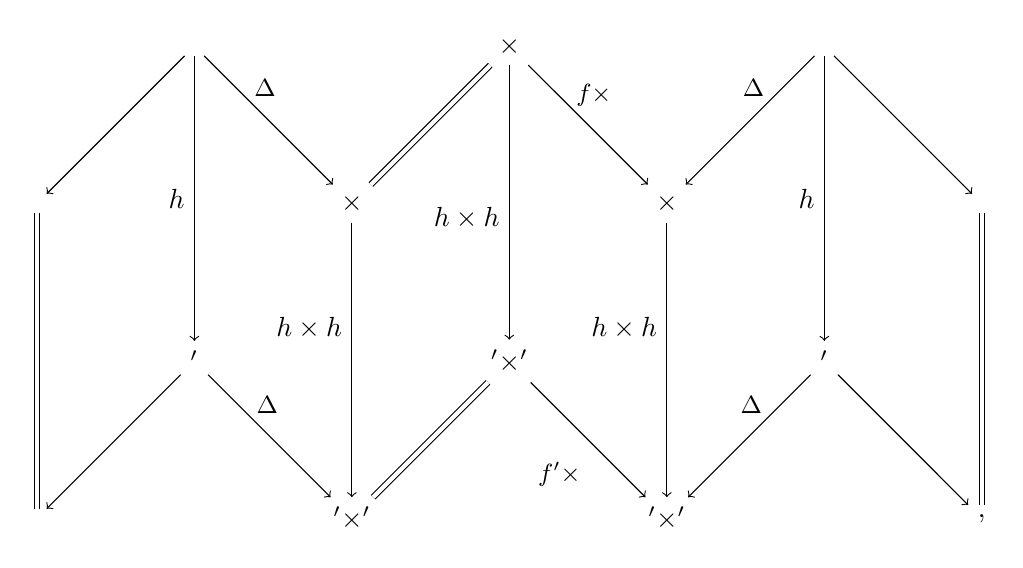
\begin{tikzpicture}[baseline=(current bounding box.center),scale=2]
      %%% Bottom diagram
      % bottom row (R0)
      \node (R0C0) at (-3,0){$\pt$};
      \node (R0C2) at (-1,0){$\tset '\times \tset '$};
      \node (R0C4) at (1,0){$\tset '\times \tset '$};
      \node (R0C6) at (3,0){$\pt$,};

      % R1
      \node (R1C1) at (-2,1){$\tset '$};
      \node (R1C3) at (0,1){$\tset '\times \tset '$};
      \node (R1C5) at (2,1){$\tset '$};

      \draw
      (R1C1) edge[->] (R0C0)
      (R1C3) edge[double distance=1.5pt] (R0C2)
      (R1C5) edge[->] node[near start,left=3pt]{{\small $\Delta$}} (R0C4)
      (R1C5) edge[->] (R0C6)
      (R1C3) edge[->] node[near start,yshift=-8mm]{{\small $f'\times\id$}}(R0C4)
      (R1C1) edge[->] node[near start ,right=3pt]{{\small $\Delta$}} (R0C2);

      %%% Top diagram
      % bottom row (R0)
      \node (newR0C0) at (-3,2){$\pt$};
      \node (newR0C2) at (-1,2){$\tset\times \tset$};
      \node (newR0C4) at (1,2){$\tset\times \tset$};
      \node (newR0C6) at (3,2){$\pt$};

      % R1
      \node (newR1C1) at (-2,3){$\tset$};
      \node (newR1C3) at (0,3){$\tset\times \tset$};
      \node (newR1C5) at (2,3){$\tset$};

      \draw
      (newR1C1) edge[->] (newR0C0)
      (newR1C3) edge[double distance=1.5pt] (newR0C2)
      (newR1C5) edge[->] node[near start,left=3pt]{{\small $\Delta$}} (newR0C4)
      (newR1C5) edge[->] (newR0C6)
      (newR1C3) edge[->] node[near start,right=3pt]{{\small $f\times\id$}}(newR0C4)
      (newR1C1) edge[->] node[near start ,right=3pt]{{\small $\Delta$}} (newR0C2);

      \draw (newR0C6) edge[double distance=1.5pt] (R0C6);
      \draw (newR1C5) edge[->] node[left]{$h$}(R1C5);
      \draw (newR1C3) edge[->] node[left,yshift=-2mm]{$h\times h$}(R1C3);
      \draw (newR1C1) edge[->]node[left]{$h$} (R1C1);
      \draw (newR0C4) edge[->]node[left,yshift=4mm]{$h\times h$} (R0C4);
      \draw (newR0C2) edge[->]node[left,yshift=4mm]{$h\times h$} (R0C2);
      \draw (newR0C0) edge[double distance=1.5pt] (R0C0);
    \end{tikzpicture}
  \]
  and taking pullbacks to compose these morphisms in the span category shows that the 2-cell identifies with
  \[
    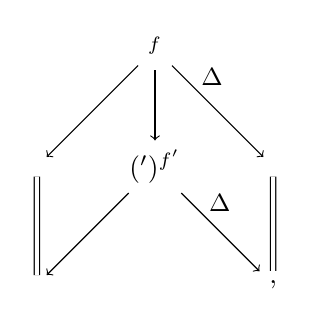
\begin{tikzpicture}[baseline=(current bounding box.center),scale=1.5]
      \node (Af) at (0,2){$\tset ^f$};
      \node (pt00) at (-1,1){$\pt $};
      \node (pt10) at (1,1){$\pt$};
      \node (Afprime) at (0,1){$(\tset ') ^{f'}$};
      \node (pt01) at (-1,0){$\pt $};
      \node (pt11) at (1,0){$\pt$,};

      \draw (Af) edge[->] (pt00);
      \draw (Af) edge[->] node[very near start,right=3pt]{{\small $\Delta$}}(pt10);

      \draw (Afprime) edge[->] (pt01);
      \draw (Afprime) edge[->] node[very near start,right=3pt]{{\small $\Delta$}}(pt11);

      \draw
      (pt01) edge[double distance=1.5pt] (pt00)
      (pt11) edge[double distance=1.5pt] (pt10)
      (Af) edge[->] (Afprime);
    \end{tikzpicture}
  \]
  where the middle vertical arrow is the restriction of $h$ to $\tset^f$.
\end{proof}

Combining this with~\cref{cor:lefschetz-triangle}, we deduce:

\begin{thm}[Lefschetz fixed point formula]\label{thm: fancy lefschetz formula}
  Let $\tset$ be a compact Hausdorff space that is locally of singular shape, and let $f\colon\tset\to\tset$ be a self-map. There is a commutative diagram
  \begin{equation}\label{eq: lefschetz-triangle-identified}
    \begin{tikzcd}[column sep=tiny]
      & \cptSections{\tset^f}\arrow[dr] \\
      \SS\arrow["L(f)", rr]\arrow[ru] && \SS,
    \end{tikzcd}
  \end{equation}
  where the bottom arrow is the Lefschetz trace of $f$ and the arrow $\SS\to\cptSections{\tset^f }$ is the one induced by the projection $\tset^f\to\pt$, or in other words the unit in the sheaf cohomology ring $\cptSections{\tset^f}\simeq\Sections{\tset^f}$.
\end{thm}
\begin{proof}
  It remains only to justify the statement about the map $\SS\to\cptSections{\tset^f}$. Recall that~\eqref{eq:lefschetz-triangle} is induced by the factorization~\eqref{eq:lax-composition-lefschetz} of the lax commutative square~\eqref{eq:lax-comm-square-lefschetz}. In this factorization, the first factor is precisely the lax square induced by the proper morphism $(\tset ,f)\to (\pt ,\id )$ as in~\eqref{eq:square-induced-by-proper-morphism}. The desired conclusion now follows from the naturality statement in~\cref{lem: trace computation}.
\end{proof}

We immediately get:
\begin{cor}[Lefschetz fixed point theorem]
  Let $A$ and $f$ be as in the previous theorem. If the Lefschetz trace of $f$ is nonzero, then $f$ has a fixed point.
\end{cor}
\begin{proof}
  If $\tset^f$ is empty, then $\cptSections{\tset^f}\simeq 0$ and so the Lefschetz trace must be null.
\end{proof}

\begin{defn}
    Let $\tset \in \Top$ be compact and locally of singular shape. For
    any self map $f\colon \tset\to \tset$, we call the map
    \[ \mdef{\lambda_f}\colon \cptSections{\tset^f}\to \SS\,, \]
    appearing as the right hand diagonal arrow in \cref{eq: lefschetz-triangle-identified}, the \tdef{topological Reidemeister trace} of $f$.
\end{defn}

Finally, we show how to recover~\cref{thm: lefschetz formula} from~\cref{thm: fancy lefschetz formula}.

\begin{proof}[Proof of \cref{thm: lefschetz formula}]
  First, note that for any compact anima $X$ and a self-map $g\colon X\to X$ we have that:
  \[
    \sum_{i\geq 0}(-1)^{i} \tr{(H^{i}(g)\curvearrowright H^{i}(\tset;\QQ )}{} = L(g)\,.
  \]
 Indeed, this is immediate since both the rationalization functor $\Sp\to \Mod_{\QQ}$ and the homotopy group functor $\pi_{\ast}\colon \Mod_{\QQ}\to \mathrm{grVect}_{\QQ}$ are symmetric monoidal.
%   is an integer, and there is a homotopy
%   \begin{equation}
%     \label{eq:trace-hurewicz}
%     \tr{g^*\curvearrowright\SS^X}{\Sp} \simeq
%     \left(\sum_{i\geq 0}(-1)^{i} \tr{(H^{i}(g)\curvearrowright H^{i}(\tset;\QQ )}{}\right)\cdot \id_\SS.
%   \end{equation}
% \end{prop}
% \begin{proof}
%   Extension of scalars along the unit map $\SS\to\QQ$ defines a symmetric monoidal functor $\QQ\otimes {-}\colon\Sp\to\Mod_{\QQ}$. Since $\QQ$ is a field, the homology functor $H_*\colon\Mod_{\QQ}\to\grVect_{\QQ}$ is symmetric monoidal,\todo{In notation and conventions should establish that graded vector spaces is given the koszul sign rule symmetric monoidal structure} and in the 1-category of graded vector spaces we calculate
%   \[
%     H_*\left( \QQ\otimes\tr{g^*\curvearrowright\SS^X}{\Sp}\right) = \sum_{i\geq 0}(-1)^{i} \tr{(H^{i}(g)\curvearrowright H^{i}(\tset;\QQ )}{}.
%   \]
%   The conclusion now follows, since $H_*(\QQ\otimes{-})\colon\pi_0\Map_{\Sp}(\SS ,\SS )\to\pi_0\Map_{\grVect_{\QQ}}(\QQ ,\QQ )$ sends $\id_\SS$ to $\id_\QQ$.

Base changing~\eqref{eq:lefschetz-triangle} along the Hurewicz map $\SS\to\QQ$ and using the projection formula $\QQ\otimes\Gamma_c(\tset^f)\simeq \Gamma_c(\tset^f;\QQ )$, we get a commutative diagram
\[
  \begin{tikzcd}
    & \Gamma_c(\tset^f;\QQ ) \arrow[dr]\\
    \QQ\arrow["L(f)",rr]\arrow[ru] &&\QQ,
  \end{tikzcd}
\]
in the derived category of $\QQ$-modules, where the bottom horizontal map is the Lefschetz trace and the map $\QQ\to\Gamma_c(\tset^f;\QQ )\simeq\Gamma (\tset^f;\QQ )$ is the unit of the sheaf cohomology ring.
Here
\[
\pi_0\Map (\Gamma_c (\tset^f;\QQ ),\QQ )\simeq H_0(\tset^f_!(\tset^f)^!\QQ ),
\]
and the right-hand side is the zeroth sheaf homology of $\tset^f$.\todo{Finish}
\end{proof}
% Let $\cC$ be a symmetric monoidal $(\infty,2)$-category with monoidal unit $\1_{\cC}\in \cC$
% and write $\Omega \cC$ for the $(\infty,1)$-category of maps $\1_{\cC}\to \1_{\cC}$.
% In~\cite{highertrace} Hoyois--Sherotzke--Sibilla construct a symmetric monoidal $(\infty,1)$-category
% $\End(\cC)$ with objects given by pairs $(X,f)$ where $X\in \cC^{\dual}$ and
% $f\colon X\to X$ is an internal left adjoint, morphisms given by lax commutative diagrams
% \[\begin{tikzcd}
%     X & Y \\
%     X & Y\,
%     \arrow["\phi", from=1-1, to=1-2]
%     \arrow["f"', from=1-1, to=2-1]
%     \arrow["g", from=1-2, to=2-2]
%     \arrow[shorten <=4pt, shorten >=4pt, Rightarrow, from=2-1, to=1-2]
%     \arrow["\phi"', from=2-1, to=2-2]
%   \end{tikzcd}\]
% in $\cC$ and monoidal unit $(\1_{\cC},\id)$.
% Moreover, they show that the assignment taking $(X,f) \in \End(\cC)$ to the trace
% $\tr{\cC}{f} \in \Omega_{\1_{\cC}}\cC$ refines to a symmetric monoidal functor
% \[ \Trc_{\cC}\colon \End(\cC)\too \Omega \cC\,.\]
% 
\subsection{Local indices}

\todo{This subsection still needs to be edited to conform with the changes in preceding subsections, such as the fact that we now already have an identification of the leftmost leg in the Russian triangle.}

Say that $\tset \in \Top$ is \tdef{suave} if the map $\tset \to \pt$ is a shape submersion in the sense
of~\cite{Volpe2023}.
In what follows, we fix a compact suave topological space $\tset \in \Top$ together with a
self map $f\colon \tset \to \tset$.

% \begin{prop}\label{prop: weak lefschetz}
%   The trace map $\tr{\Gamma_c(f)}{}\colon \SS\to \SS$ factors through the pullback
%   $\SS \to \Gamma_c(A^f)$ induced by the terminal map $A^{f}\to \pt$. In particular, if $f$ has
%   no fixed points, then $\tr{\Gamma_c(f)}{}=0$.
% \end{prop}
% \begin{proof}
%   Since $A$ is compact and suave, we have adjunctions
%   \[A^{\ast}\dashv A_{\ast}\simeq A_! \dashv A^{!} \dashv A_{!}(-\otimes \omega_A)\,,\]
%   meaning both $A^{\ast}$ and $A_!$ are internal left adjoint functors in $\Prlstf$.
%   Moreover, compactness of $\tset$ implies that $f$ is a proper map and thus we have a natural equivalence
%   $f_{\ast} \simeq f_!$. We write $\sigma \colon \tset^{\ast}\to f_{\ast}\tset^{\ast}
%   \simeq f_! \tset^{\ast}$ for the natural transformation obtained by whiskering the unit
%   $\id \to f_{\ast}f^{\ast}$ with $A^{\ast}$. With this in hand, consider the following diagram
%   in $\Endtrl(\Prlstf)$:
%   \[\begin{tikzcd}
%       {\Sp} & {\D{\tset}} & {\Sp} \\
%       {\Sp} & {\D{\tset}} & {\Sp}
%       \arrow["{\tset^\ast}", from=1-1, to=1-2] \arrow[equals, from=1-1, to=2-1] \arrow["{\tset_!}", from=1-2, to=1-3] \arrow["f_{!}",from=1-2, to=2-2] \arrow[equals, from=1-3, to=2-3] \arrow["\sigma"', Rightarrow, from=2-1, to=1-2] \arrow["{\tset^\ast}"', from=2-1, to=2-2] \arrow["\mathrm{can}"', Rightarrow, from=2-2, to=1-3] \arrow["{\tset_!}"', from=2-2, to=2-3]\,.
%     \end{tikzcd}\]
%   Unwinding the definitions, we see that the composite is given by the strongly continuous
%   $\Sp$-linear functor $\tset_!\tset^{\ast}=-\otimes \Gamma(\tset) $ together with the
%   natural transformation $\can \circ \sigma$ which, on the unit evaluates
%   to the map $\Gamma(f)\colon \Gamma(\tset)\to \Gamma(\tset)$.
%   Moreover, applying the functor $\TrcL$, we get a commutative diagram in spectra of the form
%   \[\begin{tikzcd}
%       & {\tr{f_!}{\L}} \\
%       \SS && \SS \arrow["{\TrcL(\tset_!,\can)}", from=1-2, to=2-3] \arrow["{\TrcL(\tset^{\ast},\sigma)}", from=2-1, to=1-2] \arrow["{\tr{\Gamma(f)}{}}"', from=2-1, to=2-3]\,.
%     \end{tikzcd}\]
%   By \cref{lem: trace computation}, we know that we have a natural equivalence
%   $\Gamma(\tset^f)\simeq \tr{f_!}{\L}$. Thus, it suffices to show that, under this identification, the map
%   $\TrcL(\tset, \sigma)$ is the pullback along the projection $p\colon A^{f}\to \pt$, i.e.~the unit
%   transformation $\id_{\Sp} \to p_!p^{\ast}$ evaluated at the sphere $\SS\in \Sp$. This is unsightly
%   but straightforward and will also follow from the comparison in \cref{lem: maps in triangle}.
% \end{proof}

Let us now analyze the other maps appearing in the diagram above.
The map $\TrcL(\tset^{\ast},\sigma)$ is given by the composite natural transformation
\[ \SS = \tr{\id_{\Sp}}{\L}\to \tr{A_{\ast}A^{\ast}}{\L}
  \simeq \tr{A^{\ast}A_{\ast}}{\L} \xrightarrow{\sigma} \tr{f_! A^{\ast}A_{\ast}}{\L}
  \to \tr{f_!}{\L}\,.\]
Dually, the map $\TrcL(\tset_!,\sigma)$ is given by the composite
\[ \tr{f_!}{\L}\to \tr{A^{!}A_! f_!}{\L}
  \xrightarrow{\can} \tr{A^{!}A_{!}}{\L} \simeq \tr{A_!A^{!}}{\L} \to \tr{\id_{\Sp}}{\L} =\SS\,.\]
In particular, we obtain a further factorization of the trace as

\[ \SS \to \Gamma(A) \xrightarrow{a_f} \tr{f_!}{\L} \xrightarrow{b_f} \Gamma(A;\omega_A) \to \SS\,,\]
where the left and rightmost maps are the unit and counit maps respectively.
We give an explicit construction of these maps following that of 
Kashiwara--Shapira \cite{kssheaves}.

\begin{cons}
  Write $j\colon \tset^{f}\to \tset$ for the inclusion of the fixed points, $\Delta\colon \tset \to \tset \times \tset$
  for the diagonal, $\pi_i\colon \tset \times \tset \to \tset$ for the projections and
  $\Gamma^{f}:=(f,\id)\colon \tset \to \tset\times \tset$ for the graph of $f$.
  Combining the equivalences
  \[\SS_{\tset}\simeq \Delta^{!}(\pi_{1}^{\ast}\SS_{X}\otimes \pi_{2}^{\ast}\omega_{\tset})
    \simeq \Delta^{!}\pi_{2}^{\ast}\omega_{\tset}\]
  with the unit transformation $\id \to \Gamma_{\ast}^{f}(\Gamma^{f})^{\ast}$ and the Beck--Chevalley
  equivalence $\Delta^{!}\Gamma^{f}_{\ast}\simeq j_{\ast}j^!$ we obtain a map of sheaves
  \[ \SS_{\tset} \too \Delta^{!}\Gamma^{f}_{\ast}(\Gamma^{f})^{\ast} \pi_2^{\ast}\omega_{\tset}
    \simeq \Delta^{!}\Gamma^{f}_{\ast}\omega_{\tset} \simeq j_{\ast}j^{!}\omega_{\tset}\,.\]
  Further composing with the counit of the adjunction $j_!\dashv j^!$ we obtain a diagram
  of sheaves
  \[ \SS_A\to j_{\ast}j^{!}\omega_A \to \omega_A.\]
  Taking the dual $\Dl(-)=\Hom_{\D{A}}(-,\omega_A)$ and using that $\Dl\circ j_! = j_{\ast}\circ \Dl$
  by \cref{lem:push pull dual} as well as $\Dl(\omega_A)=\SS_A$ since $A$ is suave, we get a further diagram
  of sheaves
  \[ \SS_A \xrightarrow{\alpha_f} j_{\ast}j^{\ast} \SS_{A} \xrightarrow{\beta_f} \omega_A\,.\]
  Note that, $\alpha_f$ is simply induced by the unit natural transformation
  $\id_A\to j_{\ast}j^{\ast}$.
\end{cons}

\begin{lem}\label{lem: maps in triangle}
  For any self map $f\colon \tset \to \tset$ of a compact suave space $\tset \in \Top$,
  we have natural equivalences $\Gamma(\alpha_f)=a_f$ as well as $\Gamma(\beta_f)=b_f$.
\end{lem}
\todo{Do proof}
% In particular, we learn that the map $\TrcL(A^{\ast},\sigma) \colon \SS\to \Gamma(A^f)$
% is simply the unit map in cohomology, i.e~given by pullback along the projection $A^f\to \pt$.


% \begin{defn}
%   We define the \tdef{Lefschetz trace} of $f$ as the composite map
%   \[ \mdef{\ch{}{f}}\colon \Gamma(\tset^f)\xrightarrow{b_f} \Gamma(\tset;\omega_\tset) \to \SS\,,\]
%   where the right hand map is the pushforward along the projection $\tset \to \pt$.
% \end{defn}

Note that, since $\tset$ is compact suave, the closed subspace $\tset^f\subseteq \tset$ is as
well, so we have a natural identification $\Gamma(\tset^f)^{\vee}\simeq \Gamma(\tset^f;\omega_{\tset})$. Thus, we may think of $\chi_f$ as a class in the homology
$\ch{}{f} \in H_0(\tset;\SS)= H_0(\tset;\ZZ)$, i.e.~a formal sum
\[ \ch{}{f} = \sum_{[a]\in \pi_0\tset^f} \ch{a}{f}[a] \in \ZZ[\pi_0 \tset^f]\,.\]
For any $a\in \tset^f$, we call $\mdef{\ch{a}{f}} \in \ZZ$ the \tdef{Lefschetz index} of $f$ at $a$.

\begin{lem}
  If $\tset$ is a homology manifold, meaning we have a trivialization
  $\omega_{\tset} \simeq \tset^{\ast}\SS[n]$, the sum of the indices
  is given by the intersection number of the graph with the diagonal
  \[ \sum_{[a]\in \pi_0 \tset^f} \ch{a}{f} = \#(\Gamma^f\cap \Delta)\,.\]
\end{lem}
\begin{proof}
  Cite KS
\end{proof}
\todo{Another thing that might belong in this section is something like $\chi_{f\times f'}=\chi_f\times\chi_{f'}$, just as a demonstration of how easy it is to prove things like this using the categorical framework}


%%% Local Variables:
%%% TeX-master: "main"
%%% End:
